\section{YouCook: interfacce}
di seguito si riporta l'interfaccia principale della applicazione

\begin{figure}[H]
    \centering
 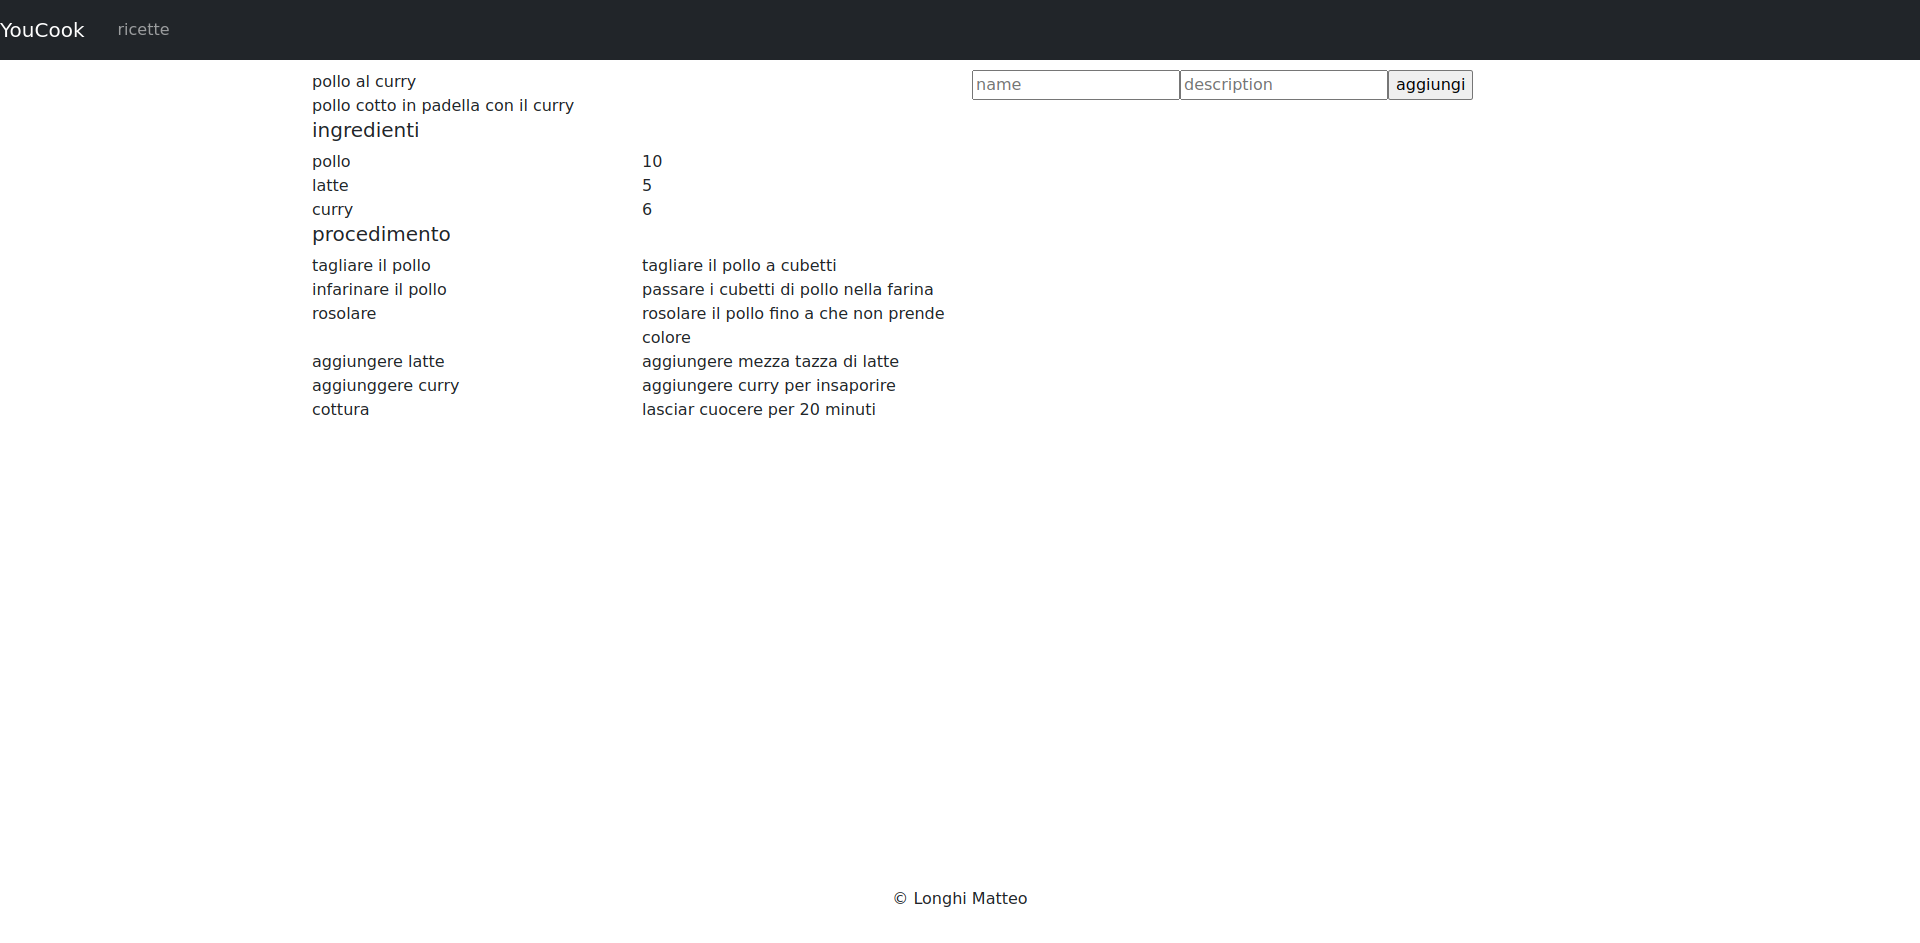
\includegraphics[scale=0.2]{resources/interfaccia-recipes.png}
   \caption{interfaccia sezione recipes dell'applicazione}
\end{figure}
L'interfaccia offre la possibilità di visionare l'elenco delle ricette e di aggiungerne di nuove tramite il form apposito.
L'elenco a destra viene renderizzato tramite la strategia onpush di change detection.
\newline
Il componente RecipesListComponent si registra a un osservabile messo a disposizione dal RecipesService che, alla modifica della lista di ricette da parte del NewRecipeComponent, emette una nuova lista di ricette attivando cosi il meccanismo di change detection
\newpage
codice NewRecipeComponent:
\begin{minted}{typescript}
import { ChangeDetectionStrategy, Component, OnInit } from '@angular/core';
import { Recipe } from '../model/Recipe';
import { RecipesService } from '../recipes.service';

@Component({
  selector: 'app-recipes-list',
  changeDetection:ChangeDetectionStrategy.OnPush,
  templateUrl: './recipes-list.component.html',
  styleUrls: ['./recipes-list.component.css']
})
export class RecipesListComponent implements OnInit {
  public recipes?:Recipe[];
  constructor(private rs:RecipesService ){
  }
  ngOnInit(): void {
   this.recipes=this.rs.getRecipes();
   this.rs.recipesEvent.subscribe(recipes=>{
    this.recipes=recipes
   })
  }
  

}

\end{minted}

\newpage
codice RecipeService;
\begin{minted}{typescript}
import { EventEmitter, Injectable } from '@angular/core';
import { DatabaseService } from 'src/database.service';
import { Recipe } from './model/Recipe';
import { SessionService } from './session.service';

@Injectable({
  providedIn: 'root'
})
export class RecipesService {
private recipes?:Recipe[];
public recipesEvent:EventEmitter<Recipe[]>=new EventEmitter();
  constructor(private dbs:DatabaseService, private ss:SessionService ) { 
    this.recipes=this.dbs.getUser(this.ss.getUsername())?.recipies;
  }
  public getRecipes(){
    return JSON.parse(JSON.stringify(this.recipes));

  }
  public addRecipes(r:Recipe ){
    this.recipes?.push(r);
   
    this.recipesEvent.emit(this.recipes);
    
  }
}
\end{minted}
